% !TEX encoding = UTF-8
% !TEX TS-program = pdflatex
% !TEX root = ../Articolo.tex
% !TEX spellcheck = it-IT

%************************************************
\section{CFDEM Characterization Workflow Coarse Particles}
\label{section:CFDemcharacterizationworkflowcoarseparticles}
%************************************************

\subsection{Pressure drop tester}
\label{subsection:pressuredroptester}

I have completed the realization of a second pressure drop tester, with a diameter 50 \% larger than the old one.
The pressure drop registered is still not reliable, the main culprits should be leakages or a wrong void ratio.\\

\subsubsection{Pressure drop tester simulation}
\label{subsubsection:pressuredroptestersimulation}

The GUI of the simulation is up and running (thx Daniel Q).
I have compared an old Nicolaus' experiment with both analytical and simulation in Fig. \ref{comparisonanalyticalexperimentsimulation}. \\

\begin{sidewaysfigure}
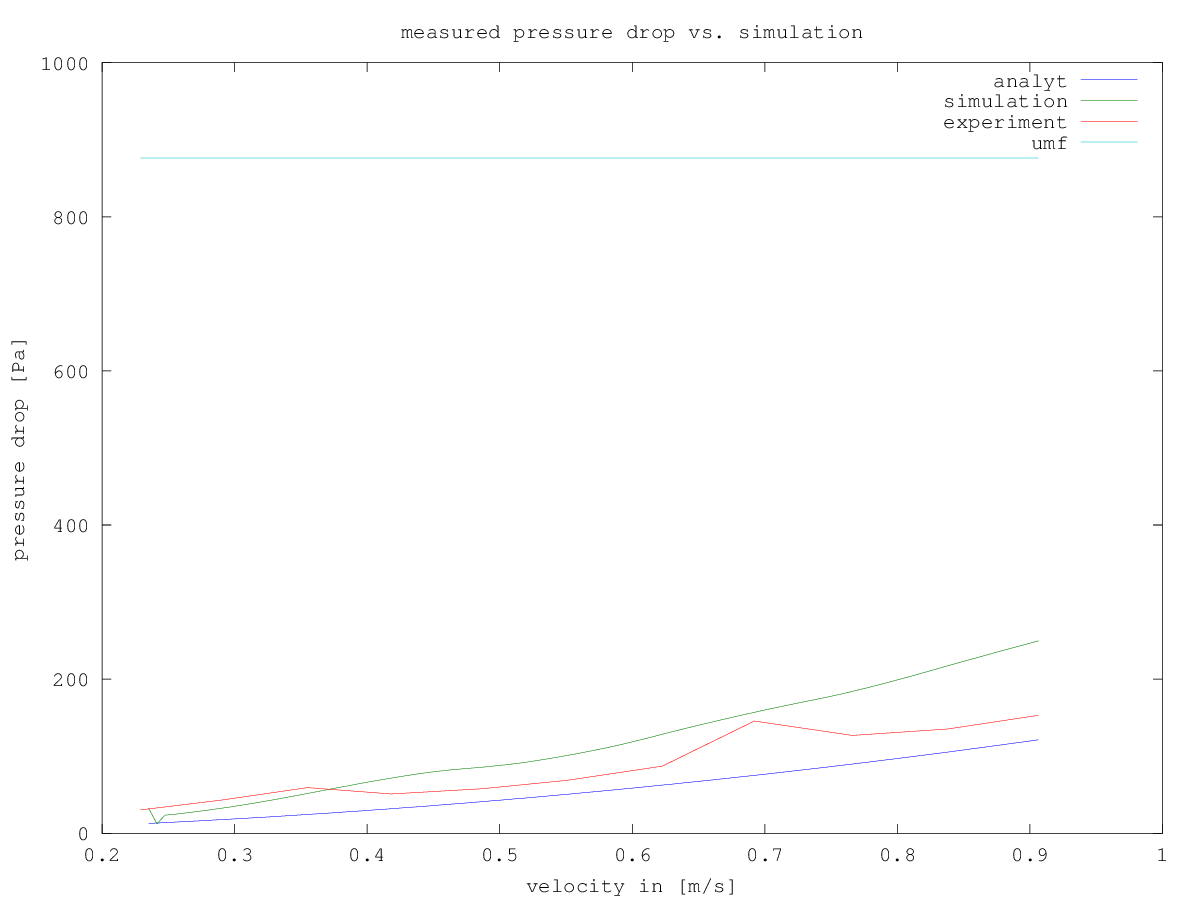
\includegraphics{009mono_glass_d2_h1300_v2_R02_xlsx_5}
\caption{mono glass d2 h1300 v2 R02 xlsx 5}
\label{comparisonanalyticalexperimentsimulation}
\end{sidewaysfigure}

\subsection{Venturi device}
\label{subsection:venturidevice}

Initially conceived as an extension of the mass hopper flow tester, I am still stuck in the design phase and I am evaluating if dropping it completely.\\